\documentclass[conference]{IEEEtran}
\IEEEoverridecommandlockouts
% The preceding line is only needed to identify funding in the first footnote. If that is unneeded, please comment it out.
\usepackage{cite}
\usepackage{amsmath,amssymb,amsfonts}
\usepackage{algorithmic}
\usepackage{graphicx}
\usepackage{textcomp}
\usepackage{subcaption}
\def\BibTeX{{\rm B\kern-.05em{\sc i\kern-.025em b}\kern-.08em
    T\kern-.1667em\lower.7ex\hbox{E}\kern-.125emX}}
\begin{document}

\title{temporary title\\
{\footnotesize CS523 Mid-Semester Report}
}

\author{\IEEEauthorblockN{Hyun Bin Lee, Aravind Sagar, Zicheng Li}

\IEEEauthorblockA{ %\textit{Department of Computer Science} \\
\textit{University of Illinois at Urbana-Champaign}\\
Urbana, United States \\
\{lee559,asagar3,zli135\}@illinois.edu}
%\and
%\IEEEauthorblockN{Aravind Sagar}
%\IEEEauthorblockA{\textit{Department of Computer Science} \\
%\textit{University of Illinois Urbana-Champaign}\\
%Urbana, United States \\
%asagar3@illinois.edu}
%\and
%\IEEEauthorblockN{Zicheng Li}
%\IEEEauthorblockA{\textit{Department of Electrical and Computer Engineering} \\
%\textit{University of Illinois Urbana-Champaign}\\
%Urbana, United States \\
%zli135@illinois.edu}
}

\maketitle

%TODO write abstract
\begin{abstract}
We propose an extension framework of Hashemi et al.'s \cite{campbell} IoT Blockchain data sharing model. While this data sharing model guarantees transparency of data sharing, users cannot confidently make a coherent decision without effectively summarizing information provided by multiple parties. We introduce a user interface for people who are willing to share data collected by IoT devices. We envision most data requests come from IoT applications as these applications potentially need access to user data to improve quality of service. Our solution assists users by providing sufficient background information to decide whether he or she should grant/deny data requests from IoT applications or explicit data requests via Messaging Service introduced in the model. Our solution is composed of i) a front-end Android application that provides an efficient summary of each data object and data request and ii) a back-end server, hosted by third-party cloud service providers, that automates communication processes among Data Owner, Data Sources and Data Requesters. Our user study shows that our user-friendly framework provides sufficient information (by whom the data was requested and which sources collected the data) and guides end-users to make autonomous decisions on potentially sensitive data.
\end{abstract}

%\begin{IEEEkeywords}
%component, formatting, style, styling, insert
%\end{IEEEkeywords}

\section{Introduction}
Smaller and more power efficient processors enables almost everything in our life to collect information and access internet. This gave rise to the idea of “Internet of Things” (IoT). 
As IoT devices prevail, our society faces many new challenges. How do we store the vast amount of data generated by these devices? How do we manage and secure them? And, most importantly, how can we help the data owners to protect their privacy? Many research efforts have been made to address the first two challenges. Among them, Sayed Hadi Hashemi has introduced a framework that allows scalable and secure manipulation of IoT data in his paper “World of Empowered IoT Devices”. However, few have been done to address the last challenge. In this paper, we further improve Sayed’s framework by introducing an intuitive way, in the form of a user interface, for the user to categorize and define access-control policies to his/her data. In addition, we see the trend of processing IoT data on cloud, we add SGX support to the framework to enforce data security in cloud computing environment.

Our main contributions include:
\begin{enumerate}
	\item While most systems tag user data from the stand point of the developers, we give users the means to tag data in a way that is intuitive to them. This, combined with an easy-to use user interface, bring the security features to an accessible level to ordinary users.

	\item By adding SGX support, we made the existing framework resilient to security concerns when using an untrusted cloud service platform.
\end{enumerate}


\section{Background}
\subsection{Internet of Things}
The term Internet of Things (IoT) originated more than 15 years ago, when it was used to describe the work of the Auto-ID Labs at the
Massachusetts Institute of Technology (MIT) on networked radio-frequency identification (RFID) infrastructures~\cite{atzori}. The definition has since expanded to beyond the scopr of RFID technologies. A lot of modern definitions have been proposed, one of them being ``a global infrastructure for the Information Society, enabling advanced services by interconnecting (physical and virtual) things based on existing and evolving interoperable information and communication technologies''~\cite{itu}.

The applications of IoT are diverse, ranging from smart industries to smart homes. In smart home area, thermostats, security systems, and energy management systems are particularly growing fast. In this paper, we focus on IoT technologies related to individual users, and these mostly fall under the smart home category, though the general principles are applicable in all areas of IoT.

Recent years have seen a rapid growth of smart devices available commercially. Ecosystems like Samsung SmartThings, Google Home and Apple Homekit are competing to become the primary player in personal IoT devices space, and for good reason -  it is estimated that IoT could grow into a market worth \$7.1 trillion by 2020~\cite{idc}.

However, the rapid expansion of IoT market also means that many issues have been overlooked, and still need resolution. Some of the relevant issues are presented in `Related Works'.

\subsection{Security and privacy in IoT (Blockchain paper)}
IoT data security is crucial in protecting user privacy. In the paper ``World of Empowered IoT Devices" \cite{campbell}, a IoT data management system is proposed. This provides a user-centric, scalable, distributed and privacy-aware system to share data between the users (data owners) and third party data requesters.

In the data management protocol of this framework, user data is stored in trusted third-party entities, known as “data sources”. IoT users are known as “data owners” to the data their devices collected. Entities who are trying to get access to user data are known as “data requesters”. 

The data owner is the only party who can grant data requesters the right, called “capability”, to access its proprietary data. When the data requester needs data access, it contacts the data owner for the capability. After acquiring the capability, the data requester will access data at data source. Throughout the process, the data owner has the control its data.

To ensure data transparency, all data transactions are recorded using BlockChains. After a successful data transaction, the data server broadcasts the transaction and the publishers update their BlockChain Record. 

\subsection{Related Works}
Davies et. al. points out that privacy concerns could be a major factor preventing wide-spread adoption of IoT devices~\cite{davies}. Over-centralization of IoT systems is identified as a critical obstacle to eliminating concern over privacy. They propose a privacy mediator which sits in between IoT devices/data and outside world, and validates permissions according to the access control policies before any data is sent out. This model includes a trusted `cloudlet', which could be a local hub or a trusted server at the edge of the cloud. They also emphasize some important characteristics that a privacy-aware IoT system should have, like exposing summarized data, user anonymity, control over inferred sensors, and ease of use. However, the model's limitation is that data storage has to happen in the sensor or the cloudlet - this could be limiting when the number of sensors increase. The model also does not discuss any framework for how to identify legitimate third party applications, and how to make sure that the request originates from the same application as it is claiming to be from.

Data mining and clustering of IoT related articles expose major problem areas in IoT~\cite{zhang}. App over-privilege, environment mistrust, LAN mistrust and weak authentication are identified as some of the problem areas that needs work. They also conclude that permissioning needs to be more fine-grained, and recommend better standards and widely-applicable systems.

Security analysis of existing IoT systems show that serious vulnerabilities exist currently~\cite{smartthings}. An analysis of Samsung Smartthings ecosystem in particular, shows that apps in the ecosystem are overpriveleged, and vulnerabilities like event spoofing can lead to privacy violation and even more serious consequences like loss of property. This goes even further in showing that a centralized proprietary system is probably not the right way to deal with IoT.


\begin{figure*}[t]

	\begin{subfigure}{0.24\textwidth}
	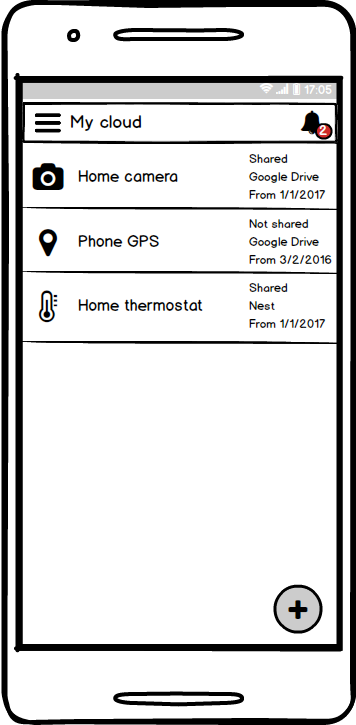
\includegraphics[width=0.95\linewidth]{screen1.png}
	\caption{Overview of user's data}
	\label{fig:screen1}
	\end{subfigure}
	\begin{subfigure}{0.24\textwidth}
	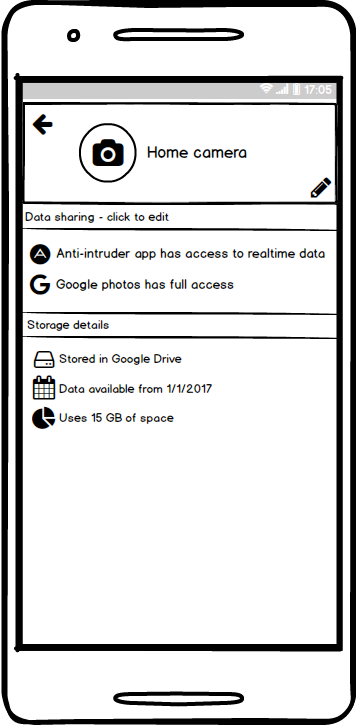
\includegraphics[width=0.95\linewidth]{screen2.png}
	\caption{Details of a particular device}
	\label{fig:screen2}
	\end{subfigure}
	\begin{subfigure}{0.24\textwidth}
	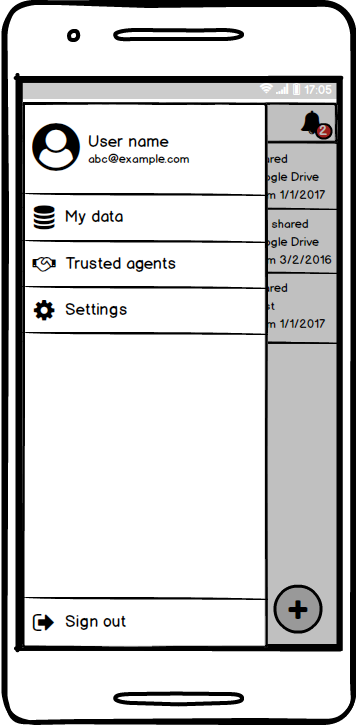
\includegraphics[width=0.95\linewidth]{screen3.png}
	\caption{Navigation drawer}
	\label{fig:screen3}
	\end{subfigure}
	\begin{subfigure}{0.24\textwidth}
	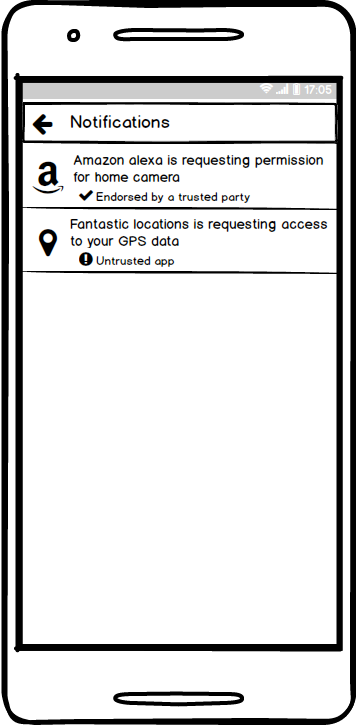
\includegraphics[width=0.95\linewidth]{screen4.png}
	\caption{Notifications screen}
	\label{fig:screen4}
	\end{subfigure}
\caption{UI mockup of the user facing application}\label{fig:screens}
\end{figure*}

\section{Problem and solution}
As evident from the previous sections, effectively addressing privacy concerns about the data generated by IoT devices is essential for the success of IoT. There are some proposed architectures which tackles this problem using user-oriented and decentralized systems. However, there's a lack of a user-facing component in such systems, which can effectively make the complex architectures usable to everyone. Our work is aimed at tackling this problem, which is "to build a user-facing component for a privacy-aware distributed user-centric IoT system (such as the blockchain based system described in \cite{campbell}), which improves the user friendliness of the system while maintaining strong security and privacy guarantees."

To accomplish this, we build the user-facing component for the blockchain based IoT architecture described in "World of empowerd IoT users \cite{campbell}". Since that system is still in development, we concentrate on the user facing components of the system, and simulate some of the external components.

The proposed work consists of 2 components:

\begin{enumerate}
	\item A smartphone app to manage IoT devices and data: Smartphones are becoming the preferred devices for internet access \cite{statcount}. Hence we build a smartphone app with which users can manage their IoT devices and data. The functionality provided by the app includes:

	\begin{enumerate}
		\item A centralized view of IoT generated data owned by them.

		\item A detailed view including the data source, access permissions and other details of this data.

		\item Permission request notifications from data requesters, and a way to accept or deny them.

		\item View, add, remove trusted parties.
	\end{enumerate}

	This is not a comprehensive list of the functionality, as we expect to add more as the project progresses. It also hides away some complexity from the users, like managing secure connection with the server described below, and managing user's private key etc. We also focus on the user-friendliness of the app, and expect to conduct user-research to find out what capabilities do users expect to find in such an app.
	
	\item A trusted server which manages the access control: This is the component which actually manages access control and capability issuance in accordance to the user's wishes. This is similar to cloudlets described in \cite{davies}, but with some key differences. First, we intend to leverage hardware technologies like Intel SGX to ensure that the server application can run on untrusted hosts. Second, this app does not store data within it; it simply interacts with the data owner, data sources and data requesters in accordance to the protocol outlined in \cite{campbell}.

	

\end{enumerate}

\section{Threat Model}
1. cellphone Trusted (we can use TrustZone based solution to be orthogonal to our solution)

2. data source Trusted

3. Endorser Trusted

4. data requesters NOT trusted

5. cloud NOT trusted

6. we are not responsible for user misassigning policies. instead we aim to minimize it

\section{Challenges}
There exists several challenges to implement our solution. We would to address these challenges in this section. 

\begin{enumerate}
\item \textbf{Simulating Roles}

Since our work is based on a theoretical model, we need to simulate each entity. During this simulation process, we may run into some implementation problems regarding details that are not explained in the literature. Thus, we need to make assumptions and augment the model in order to proceed our project. Furthermore, we may not have accurate performance benchmarks for our evaluation as we work on a simulated environment for testing our framework. 

\item \textbf{Designing User Interface}

Effective application design is an active area of research. Designing our front-end application would be the most challenging task for our project. We would like to explore Deka et al.'s~\cite{rico} large repository of mobile app design to achieve our goal for the project. Davies et al.~\cite{davies} discusses key challenges and concerns regarding how to design user policies that mediate between user and application. While they do not directly provide a clear-cut solution to the problem, authors provide a list of possible approaches to improve effectiveness of user policies.  

\item \textbf{User Study for App Interface}

The challenges related to conducting a user research for the mobile app are two fold.

First, we are building an interface for which the backend is unfamiliar, and not available yet. This means that users need to know more background information about the interface for which we seek feedback. In particular, most of the IoT systems that exist now are centralized, and provides coarse-grained permissioning. By contrast, the system that we are targeting is distributed, user-centric, and fine grained in terms of third party data access permissions. Users need to know this to provide effective feedback about the interface.

Second, IoT is still in its infancy, and it's hard to find enthusiast users of IoT devices. We overcome this by treating smartphone sensors as basic IoT devices and building a story for user interaction with the application in terms of sensor data available from smartphones.
\end{enumerate}

\section{Experiment}
TODO

\begin{thebibliography}{00}
\bibitem{davies} Davies, Nigel, et al. ``Privacy mediators: Helping iot cross the chasm.'' Proceedings of the 17th International Workshop on Mobile Computing Systems and Applications. ACM, 2016.
\bibitem{campbell} Hashemi, Sayed Hadi, et al. ``World of Empowered IoT Users.'' Internet-of-Things Design and Implementation (IoTDI), 2016 IEEE First International Conference on. IEEE, 2016.
\bibitem{zhang} Zhang, Nan, et al. ``Understanding IoT Security Through the Data Crystal Ball: Where We Are Now and Where We Are Going to Be.'' arXiv preprint arXiv:1703.09809. arXiv, 2017
\bibitem{statcount} (2016, Nov.) ``Mobile and tablet internet usage exceeds desktop for first time worldwide.'' Statcounter global stats. [Online]. Available: http://gs.statcounter.com/press/mobile-and-tablet-internet-usage-exceeds-desktop-for-first-time-worldwide (Accessed Oct 24, 2017)
\bibitem{tz} Ahmed M. Azab, et al. 2014. ``Hypervision Across Worlds: Real-time Kernel Protection from the ARM TrustZone Secure World.'' In Proceedings of the 2014 ACM SIGSAC Conference on Computer and Communications Security (CCS '14). ACM, New York, NY, USA, 90-102. DOI: http://dx.doi.org/10.1145/2660267.2660350
\bibitem{leaky} Wang, Wenhao, et al. ``Leaky Cauldron on the Dark Land: Understanding Memory Side-Channel Hazards in SGX.'' ACM Computer and Communications Security (CCS ’17), October, 2017.
\bibitem{mengjia} Yan, Mengjia, et al. 2017. ``Secure Hierarchy-Aware Cache Replacement Policy (SHARP): Defending Against Cache-Based Side Channel Atacks.'' In Proceedings of the 44th Annual International Symposium on Computer Architecture (ISCA '17). ACM, New York, NY, USA, 347-360. DOI: https://doi.org/10.1145/3079856.3080222
\bibitem{raccoon} Rane, Ashay, et al. ``Raccoon: Closing digital side-channels through obfuscated execution.'' In USENIX Security Symposium (2015).
\bibitem{atzori} Atzori, Luigi, Antonio Iera, and Giacomo Morabito. ``The internet of things: A survey." Computer networks 54.15 (2010): 2787-2805.
\bibitem{itu} (2012, Jun) ``Overview of Internet of Things.'' ITU-T Recommendations. Available: http://www.itu.int/ITU-T/recommendations/rec.aspx?rec=y.2060 (Accessed Oct 25, 2017)
\bibitem{idc} (2015, Jun) ``Internet of Things Market to Reach \$1.7 Trillion by 2020''. The Wall Street Journal. Available: https://blogs.wsj.com/cio/2015/06/02/internet-of-things-market-to-reach-1-7-trillion-by-2020-idc/ (Accessed Oct 25, 2017)

\end{thebibliography}

\end{document}